\documentclass[12pt]{report}
\usepackage{xcolor}
\usepackage{fullpage}
\usepackage{graphicx}
\usepackage{fixltx2e}
\usepackage[margin=0.5in]{geometry}
\begin{document}
	\definecolor{mycolor1}{RGB}{210,210,255}
\centering{\colorbox{mycolor1}{\textbf{\Huge{\hspace{10pt}KARTIK VASHISHT}}}

\colorbox{mycolor1}{\textbf{\Large{Electronics and Communication Engineering}}}

\vspace{7pt}
\textbf{\large{Address(Permanent): E-44 Kilokeri opp. Maharani Bagh, New Delhi-14 }}

\textbf{\large{Address(Corresponding): B-258, Hostel No.10 (Visvesvara Bhawan),\qquad}} 
			
\textbf{\large{\hspace{170pt} National Institute of Technology, Kurukshetra}}

\vspace{10pt}
\colorbox{white}{\textbf{\large{Email: karvash.kv@gmail.com \qquad \qquad Contact No.: 8295156523/9729045096}}}

\vspace{10pt}
\begin{figure}
	\centering
	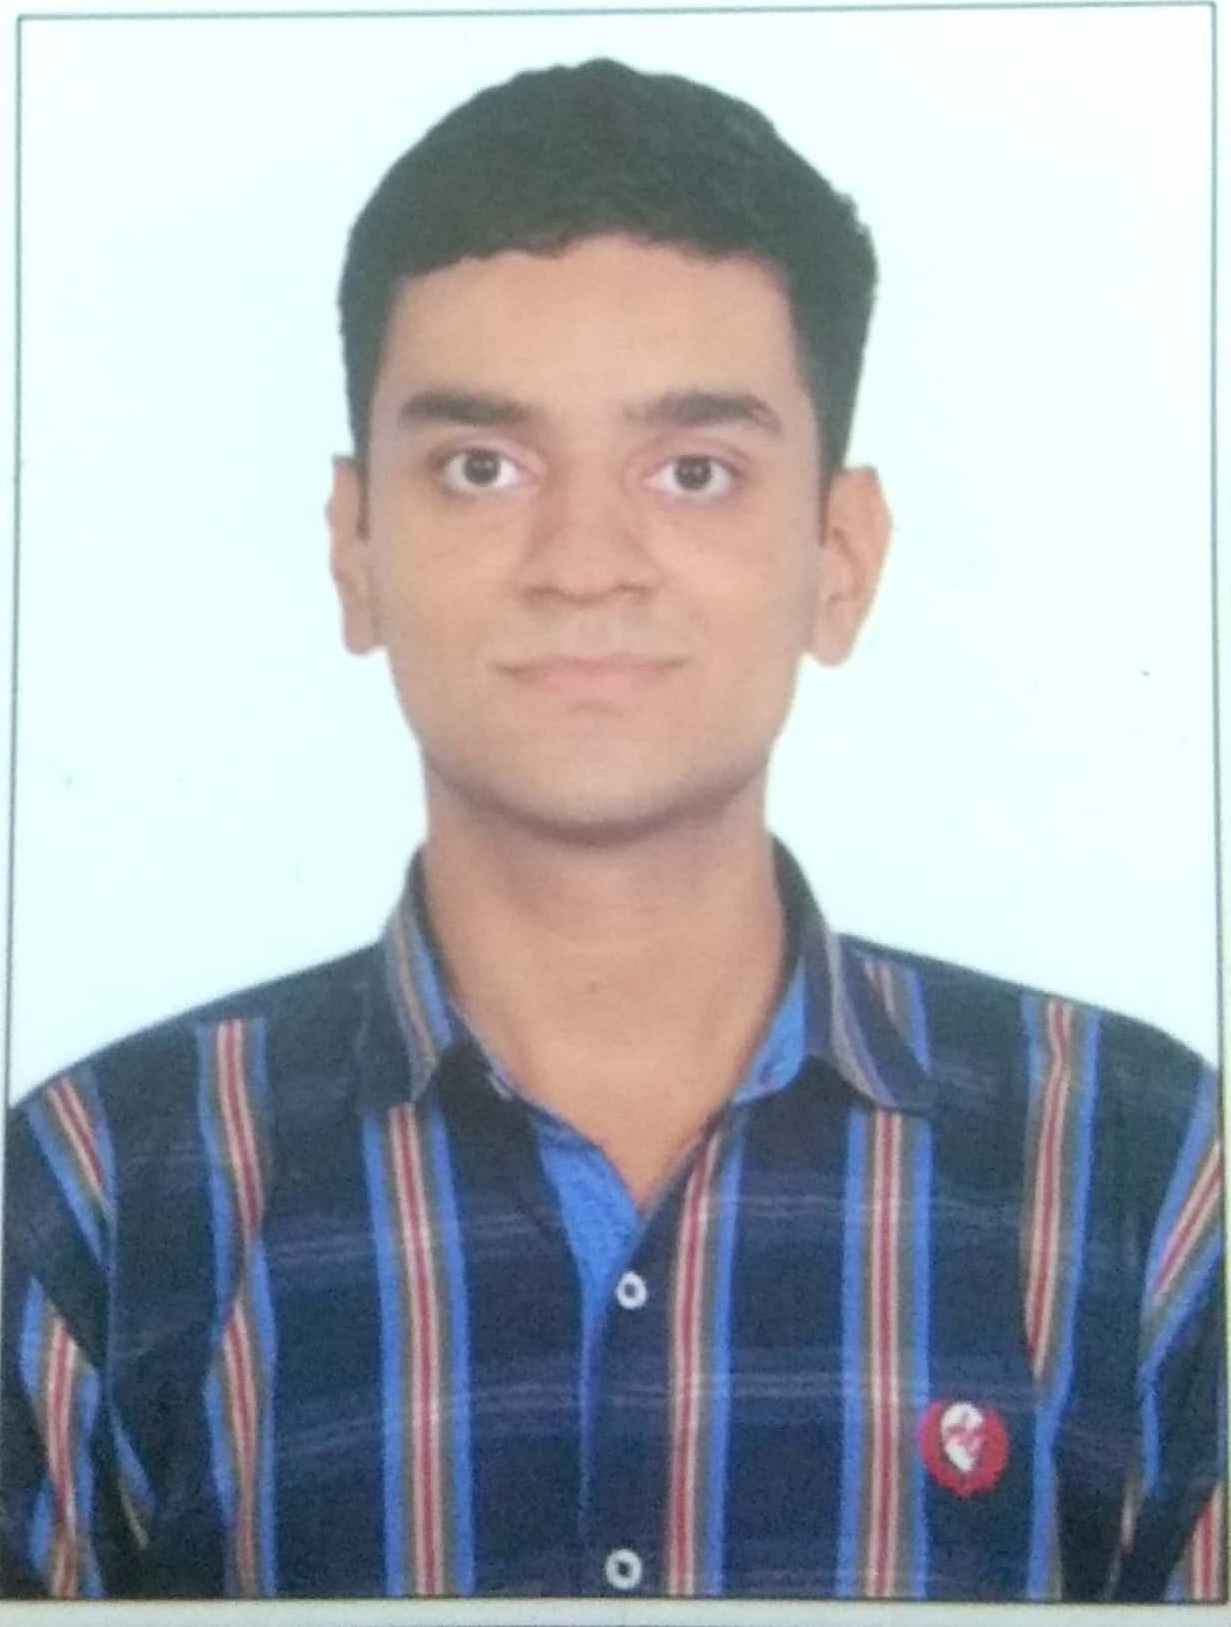
\includegraphics[scale=0.13]{Self.jpg}
\end{figure}

\vspace{20pt}
\textbf{\large{\underline{Career Objectives:}}}
\large{ The future objective and aims of my life are to gain as much knowledge as I can and use that knowledge in implementing solutions and engineering things that can help in solve in daily life problems. I am enthusiastic about electronics and communication and want to explore deep in this field. I want to contribute toward making the world a simpler, better, safer place. So I want to learn and work with new skills, fields, gadgets and experts in my future. }

\vspace{15pt}
\textbf{\large{\underline{Education:}}}

\vspace{6pt}
\begin{tabular}{||c|c|c|c|c|c|c|c||}
	\hline
	\textbf {Exam} & \textbf {Institution} & \textbf {Year of Passing} & \multicolumn{5}{ c|| }{\textbf {GPA or \%}} \\
	\hline
	B.Tech. & NIT, Kurukshetra & 2020 & \small 5\textsuperscript{th} S & \small 4\textsuperscript{th} S & \small 3\textsuperscript{rd} S & \small 2\textsuperscript{nd} S & \small 1\textsuperscript{st} S  \\ \cline{4-8}
	& & (still not & 9.0 & 9.592 & 9.4 & 9.48 & 9.14 \\ \cline{4-8}
	& & completed) & \multicolumn{5}{ c|| }{Aggregate CGPA: 9.38} \\
	\hline
	12\textsuperscript{th} Board & Navodaya Bal Sr. Sec. & 2016 & \multicolumn{5}{ c|| }{89.8\%} \\ (RBSE) & School, Kota, Rajasthan & &\multicolumn{5}{ c|| }{}\\
	\hline
	10\textsuperscript{th} Board & Cambridge School, & 2014 & \multicolumn{5}{c||}{10}\\(CBSE) & Srinivaspuri, New Delhi & &\multicolumn{5}{c||}{}\\
	\hline
\end{tabular}

\vspace{3pt}
\normalsize{. \hspace{450pt} *S - Semester}

\vspace{80pt}
\textbf{\large{\underline{Projects:}}}
\begin{enumerate}
	\large{\item Made a prototype on Smart Irrigation System based on soil moisture and temperature that can be controlled automatically and manually from a remote location.}
	\item Created a model of mocking the action of a bee using PlutoX drone under the theme Pollinator Bee in e-Yantra Robotics Competition-2018.
	\item 	Created a TIC-TAC-TOE with the help of Basic Image Processing using Python.
	\item Gesture Controlled Robot using Accelerometer and Bluetooth Sensor, controlled using remote or Self Made Mobile App (using MIT app inventor).
	\item	Obstacle Detection and Avoidance Robot using ultrasonic sensor. 
	\item Created Smart lighting, Christmas lighting, Emergency alarms and many models using Arduino.
	\item Created a Best-out-of-Waste Hydraulics bridge using syringe and ice cream sticks.
	\item Created an Electricity Generator using Dynamo and rotating wheel.
	\item Designed Line-Following Robot with and without microcontroller.
\end{enumerate}


\vspace{15pt}
\textbf{\large{\underline{Training and Internship:}}}
\begin{itemize}
		\large{\item Attended summer training in Embedded Systems and IoT using PIC microcontroller. }
	\item Enrolled in online courses on Solar Energy (by Deft University), Internet of Things (by SchoolSteps and PTC).
	\item Attended workshops on IoT using Raspberry Pi, Verilog HDL, Embedded Systems using Atmega8, Single Layer PCB designing 
\end{itemize}

\vspace{15pt}
\textbf{\large{\underline{Research Publication:}}}
\begin{enumerate}
	\large{\item Worked with few batch mates on understanding and exploring the data rate and communoication through LiFi.}
	\item Worked under the guidance of a professor in understanding the basic working and possible role of Device-to-Device Communication(D2D) on 5G.
\end{enumerate}


\vspace{205pt}
\textbf{\large{\underline{Technical Skill:}}}
\begin{itemize}
		\large{\item	Has exposure to IoT using ESP8266 and NodeMCU in Arduino IDE and ESPlorer. }
	\item Worked with Hardwares like Arduino, ESP8266, Raspberry Pi.
	\item Familiar with languages like Verilog HDL, C-Programming, Python.
	\item Worked on Image processing using Python, Photoshop, MATLAB, Proteus, Cisco Packet Tracer, ESPlorer, ModelSim. 
\end{itemize}

\paragraph{}\vspace{15pt}
\textbf{\large{\underline{Soft Skill:}}}
\begin{enumerate}
	\large{\item Dedicated towards work assigned}
	 \item Hard Working
	 \item Loyal towards goal,people and work
	 \item Politeness towards companions and peers \item Persistent in Efforts
	 \item Innovative in thinking new ways and ideas
	 \item Curious towards new things and learning
	 \item Goal Oriented
	 \item Respect people, work and emotions
	 \item Aims at completing work before time 
	 \item Tries to remain punctual in time 
	 \item Tries to find solution to any situational problem
	 \item Team Player who thinks that a team can be more efficient than an individual.
	 \item Nature Lover and Admirer
\end{enumerate}

\vspace{15pt}
\textbf{\large{\underline{Extra Curriculum Activities:}}}
\begin{itemize}
	\large{\item Playing Sports like Football, Badminton, Cricket, Table Tennis, Chess. }
	\item Listening to music. 
	\item Making Sketches of people.
	\item Writing and creating poems.
	\item Playing Piano.
	\item Talking to people and discussing on various topics.
	\item Meditating and love for traveling  
\end{itemize}

\vspace{15pt}
\textbf{\large{\underline{Co-Curriculum Activities:}}}
\begin{enumerate}
	\large{\item Surfing the internet for information related to how weapons work, how things work, what is science behind something odd and what if something changes its way of working. }
	\item Organizes robotics workshop in college
	\item Help my sister in her 12\textsuperscript{th} studies.
	\item Help in directing and working with juniors on small projects.
	\item Have frequent discussions on subjects and what is going on around the world in Science and Technology.
	\item Attending workshops, seminars and guest lectures by experts.
\end{enumerate}

\vspace{20pt}
\textbf{\large{\underline{Personal Information:}}}

\large{Father's Name: Vikas Sharma \hspace{110pt} Mother's Name: Aruna Sharma  }

\large{Date of Birth: 17-August-1998 \hspace{110pt} Gender: Male \hspace{110pt}}

\large{Place of Birth: Kota, Rajasthan \hspace{90pt} Languages Known: Hindi, English}

\large{Nationality: Indian \hspace{90pt} Marital Status: Single}

\vspace{50pt}
\textbf{\large{\underline{Reference:}}}

\large{Vineet Vashisht (Regional Sales Manager, Opple India Pvt. Ltd., 9212392023), \hspace{100pt}HL Sharma (Retired Irrigation Engineer, 9887610890), AC Sri Krishna (Companion,8295142463), Siddharth Arya (Companion,9999893851), Navjot Singh (Companion, 8811824288), Rohit Chaudhary (Senior, 7404659903)}

\end{document}